
    % First subfigure
    \begin{subfigure}[b]{0.45\textwidth}
        \centering
        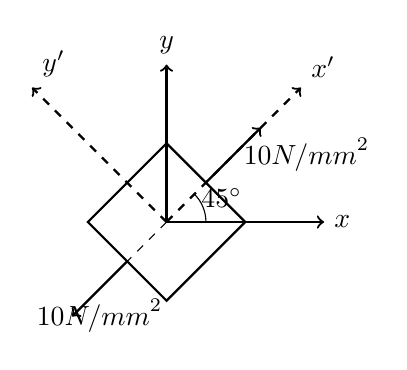
\begin{tikzpicture}
        \draw [thick,->] (0,0) -- (2,0) node[right] {$x$};
\draw [thick,->] (0,0) -- (0,2) node[above] {$y$};
\draw [thick,->,dashed] (0,0) -- (1.707,1.707) node[above right] {$x'$};
\draw [thick,->,dashed] (0,0) -- (-1.707,1.707) node[above right] {$y'$}; 
\draw [thick] (0,1) -- (1,0) -- (0,-1) -- (-1,0) -- cycle;
\draw [thick,->] (0.5,0.5) -- (1.2,1.2) node[midway,right] {$10 \text{ N/mm}^2$};
\draw [thick,->] (-0.5,-0.5) -- (-1.2,-1.2) node[midway,below] {$10 \text{ N/mm}^2$};
\draw [dashed] (0,0) -- (-0.5,-0.5);
\draw (0.5,0) arc (0:45:0.5) ;
\node at (0.7,0.3) {$45^\circ$};

            
        \end{tikzpicture}
        \caption{State of stress in case I}
        
    \end{subfigure}
    \hfill
    % Second subfigure
    \begin{subfigure}[b]{0.45\textwidth}
        \centering
        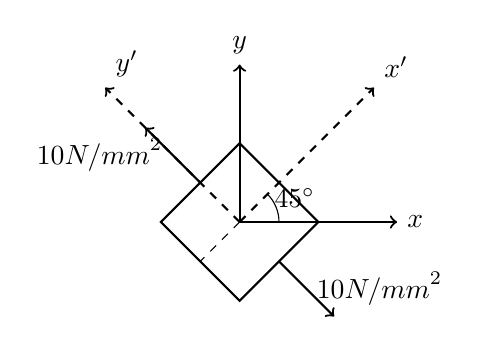
\begin{tikzpicture}
\draw [thick,->] (0,0) -- (2,0) node[right] {$x$};
\draw [thick,->] (0,0) -- (0,2) node[above] {$y$};
\draw [thick,->,dashed] (0,0) -- (1.707,1.707) node[above right] {$x'$};
\draw [thick,->,dashed] (0,0) -- (-1.707,1.707) node[above right] {$y'$}; 
\draw [thick] (0,1) -- (1,0) -- (0,-1) -- (-1,0) -- cycle;
\draw [thick,->] (0.5,-0.5) -- (1.2,-1.2) node[midway,right] {$10 \text{ N/mm}^2$};
\draw [thick,->] (-0.5,0.5) -- (-1.2,1.2) node[midway,left] {$10 \text{ N/mm}^2$};
\draw [dashed] (0,0) -- (-0.5,-0.5);
\draw (0.5,0) arc (0:45:0.5) ;
\node at (0.7,0.3) {$45^\circ$};

        \end{tikzpicture}
        \caption{State of stress in case II}
    \end{subfigure}
    \label{fig:tikz_subfigures}

